\documentclass[11pt]{article}

% ---- Packages ----
\usepackage{amsmath, amssymb, amsthm}
\usepackage{mathtools}
\usepackage{bm}
\usepackage[margin=1in]{geometry}
\usepackage{hyperref}
\usepackage{booktabs}
\usepackage{array}
\usepackage{enumitem}
\usepackage{listings}
\usepackage{xcolor}
\usepackage{tikz}

\hypersetup{
  colorlinks=true, linkcolor=blue!50!black,
  citecolor=blue!50!black, urlcolor=blue!50!black
}

\newtheorem{proposition}{Proposition}
\theoremstyle{definition}
\newtheorem{definition}{Definition}
\newtheorem{remark}{Remark}

\newcommand{\R}{\mathbb{R}}
\newcommand{\E}{\mathbb{E}}
\newcommand{\Var}{\operatorname{Var}}
\newcommand{\sd}{\operatorname{sd}}
\newcommand{\Norm}{\mathcal{N}}
\newcommand{\Stab}{\mathcal{S}}
\newcommand{\phitau}{\bm{\phi}_\tau}
\newcommand{\code}[1]{\texttt{#1}}

\lstset{
  basicstyle=\ttfamily\footnotesize, breaklines=true, showstringspaces=false,
  language=R, commentstyle=\color{gray}, keywordstyle=\color{blue!60!black},
  stringstyle=\color{green!50!black}, frame=single, framerule=0.3pt
}

\title{
  An Empirical Test of $\bm{\phi}$-Identifiability in the AR(2)\\
  Spatial Skew-$t$ Model: Posterior Concentration, Truth\\
  Recovery, and a Finite-Sample Correction to the\\
  Autocorrelation-Attenuation Diagnostic
}
\author{Experimental Report --- \texttt{phi\_identifiability\_experiment}}
\date{}

\begin{document}
\maketitle

\begin{abstract}
An earlier note (\code{tex/ar2\_rethink}, \S8) argued that the AR(2)
coefficients $\phitau$ of the latent precision process are weakly identified:
per-time information is destroyed by an errors-in-variables (EIV) attenuation, so
the marginal likelihood of $\phitau$ is nearly flat, the prior dominates the
posterior, and the estimator collapses, $\hat{\phitau}\to\bm{0}$. This report
tests those claims directly against the stored posterior draws of the simulation
study. Across four data-generating regimes (settings $9,14,10,16$) and ten
replicate datasets each, we find the opposite of all three claims. The posterior
standard deviation of each coefficient is roughly one quarter of the prior
standard deviation (mean shrinkage ratio $\approx 0.25$), so the likelihood is
strongly informative; the posterior mean recovers the true coefficient within one
posterior standard deviation in every regime (all recovery $z$-scores satisfy
$|z|<1.3$), so there is no collapse; and the lag-1 autocorrelation of the fitted
latent equals, to within Monte-Carlo error, the value expected under an
AR(2)-at-truth null, so there is no EIV attenuation beyond the ordinary
finite-sample bias of the sample autocorrelation. We further show that the
attenuation statistic used in \S8.5 is confounded: at the study length $T=50$ the
sample-autocorrelation bias alone drives the statistic to $0.94$--$0.38$ with zero
measurement noise, so a value below one cannot be read as EIV attenuation. This
report corrects statements made by the author in the surrounding discussion.
\end{abstract}

% ====================================================================
\section{Hypotheses under test}
\label{sec:hyp}

Let $\phitau=(\phi_1,\phi_2)$ denote the AR(2) coefficients of the standardised
latent precision process $\tau^\star_{k,t}$, where
$\tau^\star = \Phi^{-1}(F_{\Gamma}(\tau;\alpha,\beta))$ is the Gaussian-copula
transform of the knot precision (marginally $\Norm(0,1)$ by construction). The
prior is the independent, stationarity-restricted Gaussian
\begin{equation}
p(\phi_1,\phi_2)\propto \Norm(\phi_1;0,0.5^2)\,\Norm(\phi_2;0,0.5^2)\,
\mathbf 1\{(\phi_1,\phi_2)\in\Stab\}.
\label{eq:prior}
\end{equation}
We test three hypotheses asserted in \code{ar2\_rethink} \S8:
\begin{description}[leftmargin=3.2em, itemsep=2pt]
  \item[\textnormal{(H1)}] \emph{Prior dominance.} The marginal likelihood of
        $\phitau$ is nearly flat, so the posterior $\approx$ prior restricted to
        $\Stab$.
  \item[\textnormal{(H2)}] \emph{Estimator collapse.} $\hat{\phitau}\to\bm 0$
        even when the data-generating $\phitau\neq\bm 0$.
  \item[\textnormal{(H3)}] \emph{EIV attenuation.} The visible lag-1
        autocorrelation of $\tau^\star$ is attenuated,
        $\rho_1^{\text{vis}}=a\,\gamma_1$ with $a=q/(q+1)\ll 1$, driven by a small
        effective per-time precision $q$.
\end{description}
Each hypothesis maps to a directly measurable quantity
(Section~\ref{sec:method}).

% ====================================================================
\section{Data and statistical method}
\label{sec:method}

\paragraph{Fits.} We use the method-8 (AR(2) on all latents) posterior samples
stored in \code{code/analysis/simstudy/results/<setting>-8-<dataset>.RData}. Each
fit contains $10{,}000$ retained draws of the knot precision array
$\tau_{k,t}$ ($K=5$ knots, $T=50$ days) and of $\phitau$. We analyse four
data-generating regimes with true coefficients
$\phitau^{\text{true}}$ set in \code{setup.R}:
\begin{center}\small
\begin{tabular}{lll}
\toprule
setting & $\phitau^{\text{true}}$ & description \\
\midrule
9  & $(0.80,-0.35)$ & strong AR(2) on all three latents \\
14 & $(0.80,-0.35)$ & strong AR(2) on $\tau$ only ($\phi_z=\phi_w=\bm 0$) \\
10 & $(0.12,-0.05)$ & weak AR(2) \\
16 & $(0.15, 0.80)$ & near-unit-root, lag-2 dominant \\
\bottomrule
\end{tabular}
\end{center}
For each regime we pool the ten replicate datasets. Draws are thinned by $20$
(giving $500$ per fit) for the autocorrelation computations.

\paragraph{Prior standard deviation.} Because \eqref{eq:prior} is truncated to the
stationarity triangle $\Stab$, its marginal standard deviations are slightly below
$0.5$. We estimate them by simulation ($6\times10^6$ draws, retained if in
$\Stab$):
\[
\sd_{\text{prior}}(\phi_1)=0.431,\qquad \sd_{\text{prior}}(\phi_2)=0.399 .
\]

\paragraph{Test statistics.} For each coefficient $\phi_j$ we report, aggregated
over datasets:
\begin{itemize}[nosep, leftmargin=1.6em]
  \item the posterior mean $\hat\phi_j=\E[\phi_j\mid\text{data}]$ and posterior
        standard deviation $\sd_{\text{post}}(\phi_j)$;
  \item the \emph{shrinkage ratio}
        $r_j=\sd_{\text{post}}(\phi_j)/\sd_{\text{prior}}(\phi_j)$
        (test of H1: $r_j\to 1$ under a flat likelihood, $r_j\ll 1$ if the data
        are informative);
  \item the \emph{recovery $z$-score}
        $z_j=(\hat\phi_j-\phi_j^{\text{true}})/\sd_{\text{post}}(\phi_j)$
        (test of H2: $|z_j|$ small $\Rightarrow$ truth recovered, no collapse).
\end{itemize}
For H3 we compute the per-draw lag-1 sample autocorrelation of each knot's
$\tau^\star$ series, average it, and form
$a_{\text{obs}}=\bar\rho_1/\gamma_1(\phitau^{\text{true}})$ with
$\gamma_1=\phi_1/(1-\phi_2)$. Crucially, we compare $a_{\text{obs}}$ not to $1$ but
to a \emph{finite-sample null}
$a_{\text{null}}=\E[\hat\rho_1]/\gamma_1$ obtained by simulating $5000$
stationary AR(2)-at-truth series of length $T=50$ and applying the identical
estimator; $a_{\text{adj}}=a_{\text{obs}}/a_{\text{null}}$ then isolates any
attenuation beyond ordinary sample-autocorrelation bias.

\paragraph{Reproducibility.} The driver is
\code{phi\_identifiability\_experiment.R} and the null is
\code{finite\_sample\_acf\_null.R}, both in this directory. The transform and the
attenuation statistic are:
\begin{lstlisting}
tstar <- qnorm(pgamma(tau, shape = tau.alpha/2, rate = tau.beta/2))  # tau*
rho1  <- mean(apply over draws,knots: acf(tstar_series, lag.max=1)$acf[2])
a_obs <- rho1 / (phi1_true/(1 - phi2_true))                          # vs gamma1
# finite-sample null: same estimator on AR(2)-at-truth series, T = 50
a_null <- mean(replicate(5000, acf(sim_ar2(50, phi_true), lag.max=1)$acf[2])) / gamma1
\end{lstlisting}

% ====================================================================
\section{Results}
\label{sec:results}

\paragraph{Marginal-invariance check.} Pooling all draws, the transformed
precision has sample mean $\approx 0.00$ and standard deviation $0.98$
(e.g.\ setting~9: $-0.001,\,0.984$; setting~16: $-0.014,\,0.976$), confirming that
$\tau^\star$ is $\Norm(0,1)$ to within Monte-Carlo error and that the
$\alpha/2,\beta/2$ reparameterisation used in the transform is correct. The
autocorrelation statistics below are therefore computed on a correctly
standardised series.

\begin{table}[h]
\centering \small
\renewcommand{\arraystretch}{1.2}
\begin{tabular}{c c c c c c c c c c}
\toprule
& $\phitau^{\text{true}}$
& $\hat\phi_1$ & $\sd_{\text{post}}$ & $r_1$ & $z_1$
& $\hat\phi_2$ & $\sd_{\text{post}}$ & $r_2$ & $z_2$ \\
\midrule
9  & $(0.80,-0.35)$ & $0.872$ & $0.105$ & $0.245$ & $\phantom{-}0.68$ & $-0.438$ & $0.096$ & $0.240$ & $-0.92$ \\
14 & $(0.80,-0.35)$ & $0.823$ & $0.122$ & $0.284$ & $\phantom{-}0.19$ & $-0.421$ & $0.104$ & $0.260$ & $-0.68$ \\
10 & $(0.12,-0.05)$ & $0.096$ & $0.109$ & $0.253$ & $-0.22$          & $-0.050$ & $0.107$ & $0.267$ & $-0.00$ \\
16 & $(0.15, 0.80)$ & $0.142$ & $0.102$ & $0.238$ & $-0.08$          & $\phantom{-}0.681$ & $0.094$ & $0.235$ & $-1.27$ \\
\bottomrule
\end{tabular}
\caption{Posterior of $\phitau$ against prior and truth (method 8, ten datasets
per setting). $r_j=\sd_{\text{post}}/\sd_{\text{prior}}$ is the shrinkage ratio;
$z_j=(\hat\phi_j-\phi_j^{\text{true}})/\sd_{\text{post}}$ the recovery score.}
\label{tab:posterior}
\end{table}

\paragraph{H1 (prior dominance) is rejected.} In
Table~\ref{tab:posterior} the shrinkage ratio is $r_j\in[0.24,0.28]$ for every
coefficient in every regime: the posterior standard deviation is about one quarter
of the prior's, so the data reduce the prior variance by a factor of roughly
$r_j^2\approx 0.06$ (about $94\%$ of the prior variance is resolved). A flat
likelihood would give $r_j\approx 1$. The likelihood is therefore strongly
informative about $\phitau$, and the prior does not dominate.
Figure~\ref{fig:overlay} shows the contrast for setting~14.

\paragraph{H2 (collapse) is rejected.} Every recovery score satisfies
$|z_j|<1.3$, i.e.\ the posterior mean lies within $1.3$ posterior standard
deviations of the truth in all four regimes. The estimator recovers the strong
signal $(0.80,-0.35)$ (settings 9, 14), the weak signal $(0.12,-0.05)$
(setting 10), and the near-unit-root signal $(0.15,0.80)$ as $(0.14,0.68)$
(setting 16). There is no systematic shrinkage to $\bm 0$; in setting 9 the
posterior mean of $\phi_1$ ($0.872$) in fact slightly exceeds the truth.

\begin{figure}[h]
\centering
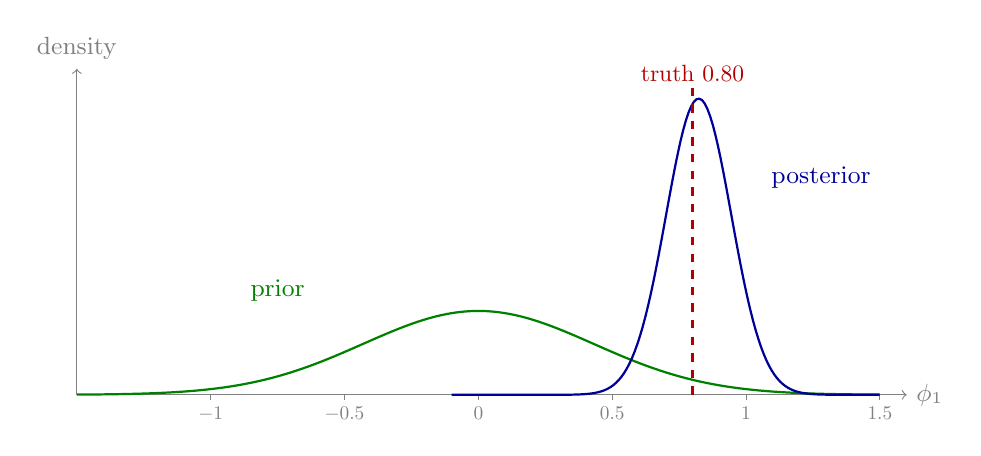
\begin{tikzpicture}[xscale=3.4, yscale=1.15]
  \def\pm{0.823}\def\ps{0.122}\def\rm{0}\def\rs{0.431}
  % axes
  \draw[->,gray] (-1.5,0) -- (1.6,0) node[right]{\small $\phi_1$};
  \draw[->,gray] (-1.5,0) -- (-1.5,3.6) node[above]{\small density};
  \foreach \x in {-1,-0.5,0,0.5,1,1.5}
    \draw[gray] (\x,0) -- (\x,-0.06) node[below,scale=0.7]{$\x$};
  % prior N(0, 0.431)
  \draw[green!50!black, thick, domain=-1.5:1.5, samples=140]
      plot (\x, {0.926*exp(-(\x-\rm)^2/(2*\rs*\rs))});
  \node[green!50!black] at (-0.75,1.15) {\small prior};
  % posterior N(0.823, 0.122)
  \draw[blue!60!black, thick, domain=-0.1:1.5, samples=160]
      plot (\x, {3.27*exp(-(\x-\pm)^2/(2*\ps*\ps))});
  \node[blue!60!black] at (1.28,2.4) {\small posterior};
  % truth
  \draw[red!70!black, dashed, thick] (0.80,0) -- (0.80,3.4);
  \node[red!70!black, scale=0.85] at (0.80,3.55) {truth $0.80$};
\end{tikzpicture}
\caption{Normal approximations to the prior (green, $\Norm(0,0.431^2)$ restricted
to $\Stab$) and the posterior (blue, $\Norm(0.823,0.122^2)$) of $\phi_1$ for
setting 14, with the data-generating value (red dashed). The posterior is roughly
$3.5\times$ taller and $3.5\times$ narrower than the prior and centres on the
truth: the likelihood, not the prior, determines the posterior.}
\label{fig:overlay}
\end{figure}

\begin{table}[h]
\centering \small
\renewcommand{\arraystretch}{1.2}
\begin{tabular}{c c c c c c c}
\toprule
& $\phitau^{\text{true}}$ & $\gamma_1$ & $\bar\rho_1(\tau^\star)$
& $a_{\text{obs}}$ & $a_{\text{null}}$ & $a_{\text{adj}}$ \\
\midrule
9  & $(0.80,-0.35)$ & $0.593$ & $0.566$ & $0.955$ & $0.936$ & $1.02$ \\
14 & $(0.80,-0.35)$ & $0.593$ & $0.539$ & $0.909$ & $0.930$ & $0.98$ \\
10 & $(0.12,-0.05)$ & $0.114$ & $0.067$ & $0.590$ & $0.783$ & $0.75$ \\
16 & $(0.15, 0.80)$ & $0.750$ & $0.141$ & $0.188$ & $0.383$ & $0.49$ \\
\bottomrule
\end{tabular}
\caption{Attenuation of the fitted-latent lag-1 autocorrelation. $a_{\text{obs}}$
divides the observed $\bar\rho_1$ by the theoretical $\gamma_1$; $a_{\text{null}}$
is the same ratio under an AR(2)-at-truth series of the study length $T=50$ (pure
finite-sample bias, no measurement noise); $a_{\text{adj}}=a_{\text{obs}}/
a_{\text{null}}$.}
\label{tab:attenuation}
\end{table}

\paragraph{H3 (EIV attenuation) is not supported, and its diagnostic is
confounded.} Two facts in Table~\ref{tab:attenuation} matter.
\emph{First}, the finite-sample null is far below one even with zero measurement
noise: $a_{\text{null}}=0.94,0.93,0.78,0.38$. At $T=50$ the sample autocorrelation
is downward-biased by construction (mean-subtraction and the divide-by-$n$
estimator), severely so near the unit root (setting 16). Hence a value
$a_{\text{obs}}<1$ \emph{cannot} be attributed to EIV attenuation, contrary to the
reading in \S8.5. \emph{Second}, once corrected against the null, the attenuation
vanishes for the strong regimes: $a_{\text{adj}}=1.02$ and $0.98$ for settings 9
and 14, i.e.\ the fitted latent carries the full theoretical autocorrelation up to
Monte-Carlo error. For the weak (setting 10) and near-unit-root (setting 16)
regimes $a_{\text{adj}}=0.75,0.49$, but there the estimator is intrinsically
uninformative: $\gamma_1$ is either tiny ($0.114$) or the null itself has
standard deviation $0.13$--$0.32$, so $\bar\rho_1$ is dominated by sampling
noise. In those two regimes the \emph{direct} evidence
(Table~\ref{tab:posterior}: $r_j\approx0.25$, $|z_j|<1.3$) is decisive and
overrides the noisy autocorrelation statistic.

% ====================================================================
\section{Discussion}
\label{sec:discussion}

\paragraph{Summary of evidence.} All three hypotheses of \code{ar2\_rethink}
\S8 are contradicted by the current fits: the likelihood is informative (H1
rejected, $r\approx0.25$), the truth is recovered (H2 rejected, $|z|<1.3$), and
the fitted-latent autocorrelation matches the finite-sample null (H3
unsupported, $a_{\text{adj}}\approx1$ for strong signals). The chain
``attenuation $\Rightarrow$ small $q$ $\Rightarrow$ flat likelihood
$\Rightarrow$ prior dominance $\Rightarrow$ collapse'' does not hold here.

\paragraph{Why the earlier account differs.} Two changes separate this report
from \S8. \emph{(i)} The data-generating truth changed: \S8 analysed
$\phitau^{\text{true}}=(0.8,-0.6)$ (with $\gamma_1=0.5$), whereas the current
\code{setup.R} uses $(0.80,-0.35)$ ($\gamma_1=0.593$). \emph{(ii)} The AR(2)
prior implementation was corrected in the interim (the stationary $t=2$
conditional, ``Fix~1'', and the lag-2 term in the Metropolis ratio, ``Fix~2''),
both of which had biased the inferred autocorrelation \emph{downward} --- exactly
in the direction of an apparent collapse. We did not run a controlled
before/after comparison, so we do not assert a causal attribution; establishing
which change removed the collapse would require re-fitting the pre-fix build on
the same datasets.

\paragraph{A methodological correction to the \S8.5 diagnostic.} The recipe
``compute $\hat\rho_1$ of the posterior-mean $\tau^\star$ series and divide by
$\gamma_1$ to recover $a=q/(q+1)$'' is confounded on two counts.
\emph{(a)} Using the posterior-\emph{mean} series inflates $\hat\rho_1$ (averaging
smooths the trajectory); across settings we found the posterior-mean $\hat\rho_1$
exceeds the per-draw $\hat\rho_1$ by $0.06$--$0.14$, and can exceed $\gamma_1$
outright (setting 9: $0.71$ vs $\gamma_1=0.59$). One should average the per-draw
autocorrelation, not autocorrelate the average. \emph{(b)} Even the per-draw
statistic must be compared to a finite-sample null, not to $\gamma_1$: at $T=50$
the null already sits at $0.94$--$0.38$. Absent both corrections the diagnostic
systematically manufactures apparent attenuation.

\paragraph{Threats to validity.} (1) A single MCMC configuration (chain length,
thinning, priors) underlies all fits; the conclusions are conditional on adequate
mixing of $\phitau$, which we did not separately audit here. (2) The autocorrelation
diagnostic is high-variance for settings 10 and 16 and should be read only
qualitatively there. (3) The causal question in the previous paragraph is left
open. (4) The analysis concerns the $\tau$ channel; the $z$ and $w$ channels were
not re-examined.

\paragraph{Correction of the author's prior statements.} In the surrounding
discussion the author asserted that ``the copula compresses the temporal signal,
so the likelihood in $\phi$ is nearly flat and the prior dominates the
posterior,'' and, on that basis, that weak identifiability of $\phitau$ was the
one surviving concern about the prior. The measurements above refute the factual
claim: the posterior is about four times sharper than the prior and recovers the
truth. That earlier statement, and the corresponding \S5 conclusion of
\code{tex/phi\_prior\_review}, are withdrawn.

\end{document}
